\documentclass{article}

% Language setting
% Replace `english' with e.g. `spanish' to change the document language
\usepackage[english, russian]{babel}
\usepackage{listings}
% Set page size and margins
% Replace `letterpaper' with `a4paper' for UK/EU standard size
\usepackage[letterpaper,top=2cm,bottom=2cm,left=3cm,right=3cm,marginparwidth=1.75cm]{geometry}
\usepackage{amsmath,amsfonts,amssymb,amsthm,mathtools}
\usepackage{hyperref}
% Useful packages
\usepackage{amsmath}
\usepackage{graphicx}
\usepackage[colorlinks=true, allcolors=blue]{hyperref}
\usepackage{titlepic}
\usepackage{graphicx}
\graphicspath{{./pictures/}}


\documentclass[11pt,a4paper]{report}
\usepackage{tcolorbox}
\tcbuselibrary{minted,breakable,xparse,skins}

\definecolor{bg}{gray}{0.95}
\DeclareTCBListing{mintedbox}{O{}m!O{}}{%
    breakable=true,
    listing engine=minted,
    listing only,
    minted language=#2,
    minted style=default,
    minted options={%
        linenos,
        gobble=0,
        breaklines=true,
        breakafter=,,
        fontsize=\small,
        numbersep=8pt,
        #1},
    boxsep=0pt,
    left skip=0pt,
    right skip=0pt,
    left=25pt,
    right=0pt,
    top=3pt,
    bottom=3pt,
    arc=5pt,
    leftrule=0pt,
    rightrule=0pt,
    bottomrule=2pt,
    toprule=2pt,
    colback=bg,
    colframe=orange!70,
    enhanced,
    overlay={%
        \begin{tcbclipinterior}
            \fill[orange!20!white] (frame.south west) rectangle ([xshift=20pt]frame.north west);
        \end{tcbclipinterior}},
    #3}


\begin{document}

    \begin{center}
        \begin{huge}
            Глобальные градиентные методы оптимизации\\
        \end{huge}

        \vspace{1.8cm}
        \includegraphics[scale=0.3]{logo-vshe}

        \vspace{7cm}

        Факультет компьютерных наук\\
        Прикладная математика и информатика\\
        г. Москва\\

        \vspace{1cm}
        Судаков Илья Александрович\\
        Февраль 2023\\
    \end{center}
    \newpage
    \tableofcontents




    \newpage


    \section{Введение}

    \subsection{Мотивация}
    Многие методы оптимизации (координатный спуск, градиентный спуск, метод сопряженного гадиента и др.) используют так называемый локальный поиск, т.е. поиск минимума одномерной функции вдоль луча в n-мерном евклидовом пространстве. При этом всегда находится локальный минимум. В проекте предлагается исследовать потенциал применения методов глобальной одномерной оптимизации для организации линейного поиска. В каких случаях удастся найти глобальной минимум многомерной функции, используя глобальный линейный поиск в контексте классических градиентных методов.

    \subsection{Задачи проекта}
    \begin{itemize}
        \item Программная реализация методов глобального линейного поиска.
        \begin{itemize}
            \item Метод Золотого сечения
            \item Алгоритм Moore-Skelboe
        \end{itemize}
        \item Реализация алгоритма оптимизации многомерной функции.
        \begin{itemize}
            \item Координатный спуск
            \item Градиентный спуск
        \end{itemize}
        \item Экспериментальное и теоретическое исследование.
    \end{itemize}

    \subsection{Цели проекта}
    Написать алгоритм, который будет находить глобальный минимум многомерной непрерывной функции:
    \begin{itemize}
        \item с хорошей скоростью
        \item с заданной точностью
        \item не хуже классических методов для унимодальных функций
    \end{itemize}

    \subsection{Ссылка на материалы}
    Ссылка на репозиторий, с разработанными материалами:\\
    \href{https://github.com/sudakovcom/global-optimization.git}{https://github.com/sudakovcom/global-optimization.git}








    \newpage


    \section{Градиентный спуск}
    Рассмотрим первый классический метод оптимизации:\\
    Пусть целевая функция имеет вид:
    $F(\vec{x}): \mathbb{X} \rightarrow \mathbb{R}$\\\\
    Задача оптимизации задана в следующем виде:
    $F(\vec{x}) \rightarrow    \underset{\vec{x} \in \mathbb{X}}{\min}$\\\\
    Основная идея метода заключается в том, чтобы идти в направлении наискорейшего спуска, а это направление задаётся антиградиентом $-\nabla F$\\\\
    и $\vec{x}^{[j+1]}=\vec{x}^{[j]}-\lambda^{[j]} \nabla F\left(\vec{x}^{[j]}\right)$
    где $\lambda ^{[j]}$ задает скорость градиентного спуска и может быть выбрана как
    \begin{itemize}
        \item постоянная, тогда метод может не сходиться
        \item убывать по какому-то закону
        \item гарантировать наискорейший спуск
    \end{itemize}

    \subsection{Алгоритм градиентного спуска}
    \begin{itemize}
        \item Задают начальное приближение и точность расчёта: $X_0, \varepsilon$
        \item Рассчитывают $\vec{x}^{[j+1]}=\vec{x}^{[j]}-\lambda^{[j]} \nabla F\left(\vec{x}^{[j]}\right)$
        \item Проверяют условие остановки (на усмотрение):
        \begin{itemize}
            \item $|x^{[j]}-x^{[j+1]}|<\varepsilon$
            \item $|F(x^{[j]})-F(x^{[j+1]})|
            <\varepsilon$
            \item $\nabla F(x^{[i]})<\varepsilon$
            \item иначе переходят к пункту 2
        \end{itemize}
    \end{itemize}

    Этот алгоритм будет реализован на python

    \subsection{Метод наискорейшего спуска}
    В случае наискорейшего спуска $\lambda^{[j]}$ определяется как:\\
    \begin{gather*}
        \lambda^{[j]}=\operatorname{argmin}_\lambda F\left(\vec{x}^{[j+1]}\right)=\operatorname{argmin}_\lambda F\left(\vec{x}^{[j]}-\lambda \nabla F\left(\vec{x}^{[j]}\right)\right)
    \end{gather*}
    чтобы вычислить $\lambda^{[j]}$ будем использовать метод золотого сечения и алгоритм Moore-Skelboe










































    \newpage



    \newpage


    \section{Координатный спуск}

    Расмотрим более простой метод оптимизации, очень похожий на градиентный спуск, который последовательно проводит минимизацию функции вдоль координатных направлений. На очередной итерации, алгоритм фиксирует все координаты, кроме той, вдоль которой будет осуществляться поиск. Так как выбор направления на каждой итерации детерменирован, то нет необходимости наличия производных у функции.\\


    Пусть целевая функция имеет вид:
    $F(\vec{x}): \mathbb{X} \rightarrow \mathbb{R}$\\\\
    Задача оптимизации задана в следующем виде:
    $F(\vec{x}) \rightarrow    \underset{\vec{x} \in \mathbb{X}}{\min}$\\\\

    \subsection{Алгоритм}
    \begin{itemize}
        \item Задают начальное приближение и точность расчёта: $X_0, \varepsilon$
        \item Рассчитывают ${\displaystyle x_{i}^{k+1}={\underset {y\in \mathbb {R} }{\operatorname {arg\,min} }}\;f(x_{1}^{k+1},\dots ,x_{i-1}^{k+1},y,x_{i+1}^{k},\dots ,x_{n}^{k})}$
        \item Проверяют условие остановки (на усмотрение):
        \begin{itemize}
            \item $|x^{[j]}-x^{[j+1]}|<\varepsilon$
            \item $|F(x^{[j]})-F(x^{[j+1]})|<\varepsilon$
            \item иначе переходят к пункту 2
        \end{itemize}
    \end{itemize}

    Таким образом, на каждой итерации будет выполнено
    ${\displaystyle F({x} ^{0})\geqslant F({x} ^{1})\geqslant F({x} ^{2})\geqslant \dots .}$\\

    Чтобы найти ${\displaystyle x_{i}^{k+1}={\underset {y\in \mathbb {R} }{\operatorname {arg\,min} }}\;f(x_{1}^{k+1},\dots ,x_{i-1}^{k+1},y,x_{i+1}^{k},\dots ,x_{n}^{k})}$ будем использовать так же метод золотого сечения и алгоритм глобальной одномерной оптимизации.













    \newpage


    \section{Метод золотого сечения}

    \subsection{Описание}

    Метод золотого сечения — это эффективная реализации троичного поиска, служащего для нахождения минимума/максимума унимодальной функции на отрезке. Лучше тем, что на каждой итерации вычисляется значение в одной, а не двух точках.\\\\
    Пусть хотим найти минимум на отрезке $[a, b]$, тогда разобьем его на 3 части 2 точками $s_1, s_2$, так чтобы при отсекании одного из крайних подотрезков, одна из точек осталась границей подотрезков, а соотношение длин подотрезков оставалось прежним.\\
    $|[a, s_1]|=|[s_2, b]|=l_1$\\
    $|[s_1, s_2]|=l_2$\\
    тогда: $\frac{l_2}{l_1}=\frac{l_1-l_2}{l_2} \Rightarrow l_1^2-l_1\cdot{l_2}-l_2^2=0 \Rightarrow \frac{l_1}{l_2}=\frac{1+\sqrt{5}}{2}=\phi$

    \subsection{Алгоритм тернарного поиска}
    написать ли

    \subsection{Оценка сложности}
    Так как на каждой итерации длина рассматриваемого отрезка умножается на $\frac{l_1+l_2}{l_1+l_2+l_2}=\frac{3+\sqrt{5}}{4+2\sqrt{5}}=\phi^{-1}$, то для достижения точности $\delta$ потребуется $\frac{\ln(\frac{|[a, b]|}{\delta})}{\ln(\phi)} \approx 2\ln(\frac{|[a, b]|}{\delta})$ итераций.

    \subsection{Применение}
    А что если функция не унимодальная, тогда к чему сойдется этот метод? К точке, которая является одним из локальных минимумов функции либо одному из концов, в котором производная неположительная.\\









    \newpage


    \section{Глобальная одномерная оптимизация}
    Алгоритм поиска глобального минимума функции вдоль одного направления будет основываться на интервальном анализе. Перечислим основные определения и теоремы, которые нам пригодятся для посторения алгоритма.

    \subsection{Определение}
    Интервалом $[a, b]$ называется следующее множество:
    \begin{gather*}
    [a,b]
        :=\{x \in \mathbb{R} | a \le x \le b\}
    \end{gather*}

    \subsection{Арифметические свойства интервалов}
    \begin{itemize}

        \item {$\bold{x} + \bold{y} =$ {${\bold{\underline{x}} + \bold{\underline{y}},  \bold{\overline{x}} + \bold{\overline{y}}}$}}

        \item {$\bold{x} - \bold{y} =$ {${\bold{\underline{x}} - \bold{\overline{y}},  \bold{\overline{x}} - \bold{\underline{y}}}$}}

        \item {$\bold{x} \cdot \bold{y} =$ {${min(\bold{\underline{x} \underline{y}}, \bold{\underline{x} \overline{y}}, \bold{\overline{x} \underline{y}}, \bold{\overline{x} \overline{y}}) , max(\bold{\underline{x} \underline{y}}, \bold{\underline{x} \overline{y}}, \bold{\overline{x} \underline{y}}, \bold{\overline{x} \overline{y}}) }$}}

        \item {$\bold{x} \div \bold{y} =$ $\bold{x} \cdot[1/\bold{\overline{y}}, 1/\bold{\underline{y}}]$, если $0 \not\in y$}

    \end{itemize}

    \subsection{Основная теорема интервальной арифметики}
    Пусть $f(x_1, ..., x_n)$ - рациональная функция вещественных аргументов $x_1, ..., x_n$, и для нее определен результат $\bold{F(X_1, ..., X_n)}$ подстановки вместо аргументов интервалов их изменения $(X_1, ..., X_n) \subset \mathbb{R}^n$ и для $(X_1, ..., X_n)$ операциии выполняются по правилам интервальной арифметики. Тогда
    \begin{gather*}
        \{f\{x_1,...,x_n\} | x_1 \in \bold{X_1},...,x_n \in \bold{X_n}\} \subset \bold{F(\bold{X_1},...,\bold{X_n}})
    \end{gather*}

    \subsection{Утверждение}

    Пусть $f(x_1, ..., x_n)$ - рациональная функция вещественных аргументов $x_1, ..., x_n$, и $\bold{F(X_1, ..., X_n)}$ соответствующая ей интервальная функция, тогда выполняется монотонность по включению.
    Пусть $\bold{X_1},...,\bold{X_n}$ и $\bold{Y_1},...,\bold{Y_n}$, такие что $\bold{X_1} \subset \bold{Y_1},...,\bold{X_n} \subset \bold{Y_n}$, тогда
    \begin{gather*}
        f\{\bold{X_1},...,\bold{X_n}\} \subset f\{\bold{Y_1},...,\bold{Y_n}\}
    \end{gather*}

    \subsection{Определение}

    Пусть $N > 0$  натуральное число. Тогда если $\langle S_0,..., S_{n-1} \rangle$ семейство непустых подмножеств множества $S$, тогда будем называть его разбиением множества $S$. В частности, обьединение $S_0,..., S_{n-1}$ равно $S$ , тогда последовательность $\langle S_0,..., S_{n-1} \rangle$ является покрытием $S$ .

    \subsection{Теорема}

    Рассмотрим задачу безусовной глобальной оптимизации. Пусть $\langle B_0,..., B_{n-1} \rangle$ семейство множеств, содержащее глобальный минимум, такое что упорядочено по возрастанию нижней границы $f(B_i)$ для $i=0, 1, 2,..., N-1$. Пусть $U$ наименьшая из верхних значений функции для подмножеств $\langle f(B_0),..., f(B_{n-1}) \rangle$. Тогда интервал $[lb(f(B_0)), U]$ содержит глобальным минимум $\mu$.


    Используя данные факты напишем алгоритм поиска глобального минимума вдоль направления.
























    \newpage
    \newpage


    \section{Алгоритм Moore-Skelboe}
    Ниже приведена реализация глобального линейного поиска, основанная на интервальном анализе
    \begin{mintedbox}{python}
        def MooreSkelboe(func_index, index, a, b, p, e_d, e_f): # func_index(number of function in list of functions), index(index of direction),
        # a(left border), b(right border), p(current point), e_d(error of d), e_f(error of f)
        F = Functions[func_index * 2 + 1]
        interval_d = []
        for i in range(len(p)):
        interval_d.append(interval[p[i], p[i]])
        interval_d[index] = interval[a, b]

        interval_f = F(interval_d)
        set_of_intervals = [[interval_d, interval_f]]
        U = right(interval_f)
        w_f = right(interval_f) - left(interval_f)
        w_d = right(interval_d[index]) - left(interval_d[index])
        best_interval = set_of_intervals[0]
        while (w_d > e_d) | (w_f > e_f):
        set_of_intervals.pop(0)
        mid_p = mid(best_interval[0][index])
        interval_1 = best_interval[0].copy()
        interval_2 = best_interval[0].copy()
        interval_1[index] = interval[left(best_interval[0][index]), mid_p]
        interval_1_f = F(interval_1)
        interval_2[index] = interval[mid_p, right(best_interval[0][index])]
        interval_2_f = F(interval_2)
        U = min(U, right(interval_1_f))
        U = min(U, right(interval_2_f))

        for i in range(len(set_of_intervals)):
        if U < left(set_of_intervals[i][1]):
        set_of_intervals = set_of_intervals[:i]
        break

        set_of_intervals.append([interval_1, interval_1_f])
        set_of_intervals.append([interval_2, interval_2_f])

        set_of_intervals.sort(key=lambda item: left(item[1]))
        best_interval = set_of_intervals[0]
        w_f = right(best_interval[1]) - left(best_interval[1])
        w_d = right(best_interval[0][index]) - left(best_interval[0][index])

        best_point = []
        for i in range(len(p)):
        best_point.append(mid(best_interval[0][i]))

        return best_point
    \end{mintedbox}
    \newpage


    \section{Тестирование}
    Ниже приведены результаты тестирования двух методов оптимизации на тестовых функциях, первый использует метод золотого сечения, для поиска минимума вдоль направления, а другой алгоритм Moore-Skelboe.

    \subsection{Функция Растригина}

    \subsubsection{График функции при $n=2$}
    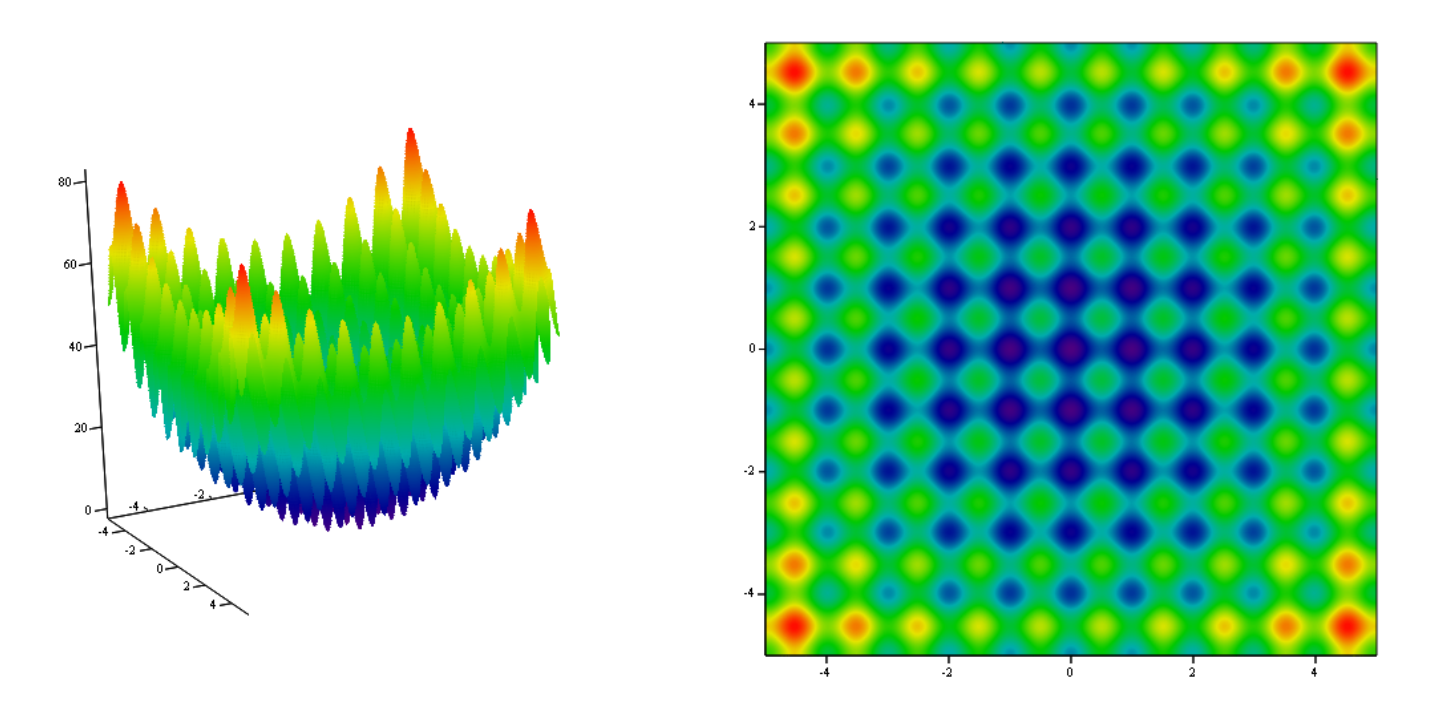
\includegraphics[width=16cm, height=8cm]{Rastrigin}

    \subsubsection{Формула}
    \begin{gather*}
        f(x)=10 n+\sum_{i=1}^n\left(x_i^2-10 \cdot \cos \left(2 \pi \cdot x_i\right)\right)
    \end{gather*}

    \subsubsection{Результаты тестирования}

    \begin{tabular}{ |p{2cm}|p{2cm}|p{3cm}|p{2cm}|p{4cm}|  }
        \hline
        n  & точность & метод         & время   & минимум                \\
        \hline
        5  & $10^-3$  & Golden ratio  & 2.22 ms & 4.974821275706137      \\\cline{2-5}
        & $10^-3$  & Moore-Skelboe & 178 ms  & 9.238348694395881e-05  \\
        \hline
        10 & $10^-3$  & Golden ratio  & 4.78 ms & 9.94964255141227       \\\cline{2-5}
        & $10^-3$  & Moore-Skelboe & 736 ms  & 0.00018476697390212848 \\
        \hline
        20 & $10^-3$  & Golden ratio  & 13.3 ms & 19.899285102824635     \\\cline{2-5}
        & $10^-3$  & Moore-Skelboe & 2.52 s  & 0.0003695339478184678  \\
        \hline
        30 & $10^-3$  & Golden ratio  & 24.1 ms & 29.84892765423696      \\\cline{2-5}
        & $10^-3$  & Moore-Skelboe & 5.38 s  & 0.0005543009217348072  \\
        \hline
        40 & $10^-3$  & Golden ratio  & 43.2 ms & 39.79857020564907      \\\cline{2-5}
        & $10^-3$  & Moore-Skelboe & 9.58 s  & 0.0007390678956511465  \\
        \hline
        50 & $10^-3$  & Golden ratio  & 58.8 ms & 49.748212757061154     \\\cline{2-5}
        & $10^-3$  & Moore-Skelboe & 14.9 s  & 0.0009238348695674858  \\
        \hline

    \end{tabular}

    \subsection{Функция Растригина новгородская}

    \subsubsection{График функции при $n=2$}
    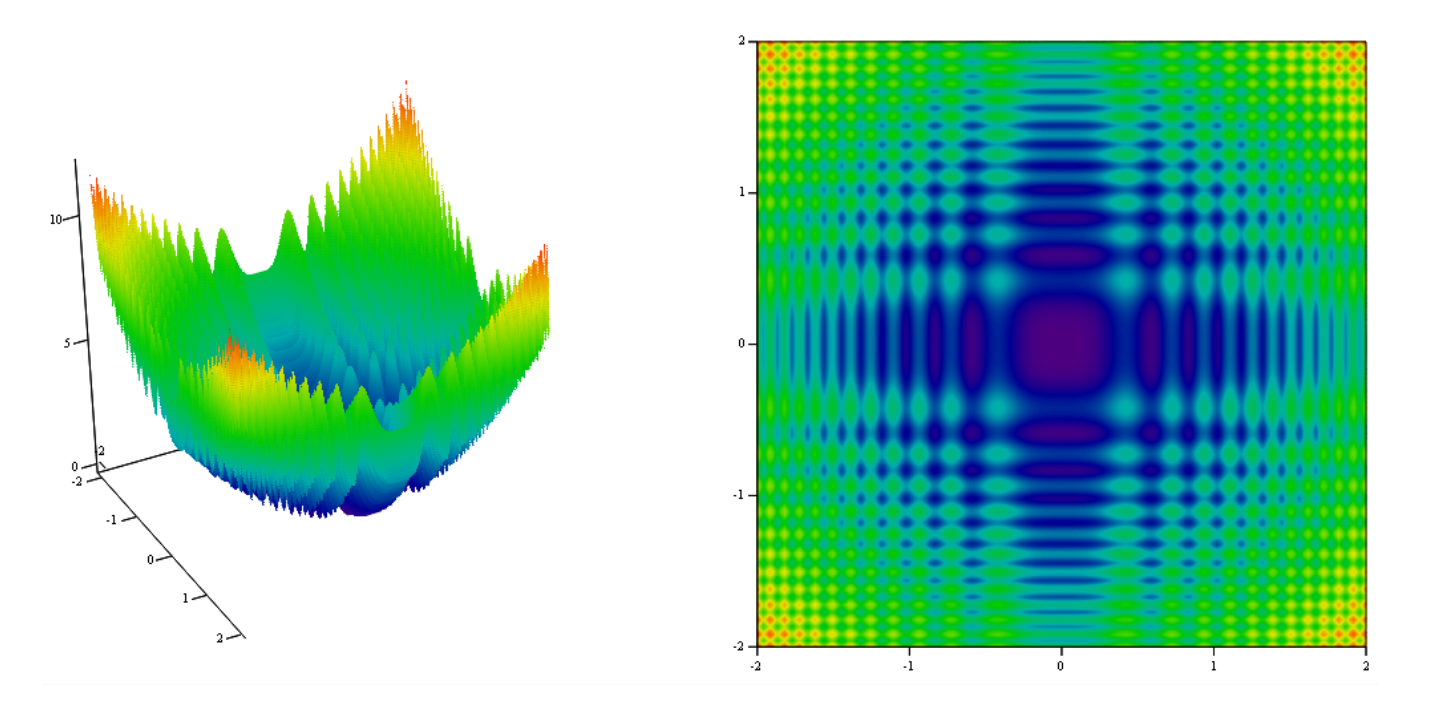
\includegraphics[width=16cm, height=8cm]{Rastrigin_new}

    \subsubsection{Формула}
    \begin{gather*}
        f(x)=n+\sum_{i=1}^n\left(x_i^2-\cos \left(18 \cdot x_i^2\right)\right)
    \end{gather*}

    \subsubsection{Результаты тестирования}

    \begin{tabular}{ |p{2cm}|p{2cm}|p{3cm}|p{2cm}|p{4cm}|  }
        \hline
        n  & точность & метод         & время   & значение              \\
        \hline
        5  & $10^-3$  & Golden ratio  & 1.36 ms & 1.542458003137213     \\\cline{2-5}
        & $10^-3$  & Moore-Skelboe & 151 ms  & 0.0007449817996270092 \\
        \hline
        10 & $10^-3$  & Golden ratio  & 5.18 ms & 3.0849160062744287    \\\cline{2-5}
        & $10^-3$  & Moore-Skelboe & 636 ms  & 0.0014899635992544624 \\
        \hline
        20 & $10^-3$  & Golden ratio  & 20.8 ms & 6.16983201254885      \\\cline{2-5}
        & $10^-3$  & Moore-Skelboe & 1.94 s  & 0.002979927198509369  \\
        \hline
        30 & $10^-3$  & Golden ratio  & 37 ms   & 9.254748018823253     \\\cline{2-5}
        & $10^-3$  & Moore-Skelboe & 4.54 s  & 0.0044698907977642754 \\
        \hline
        40 & $10^-3$  & Golden ratio  & 54.2 ms & 12.339664025097658    \\\cline{2-5}
        & $10^-3$  & Moore-Skelboe & 7.79 s  & 0.005959854397019182  \\
        \hline
        50 & $10^-3$  & Golden ratio  & 79.7 ms & 15.424580031372061    \\\cline{2-5}
        & $10^-3$  & Moore-Skelboe & 11.6 s  & 0.0074498179962740885 \\
        \hline

    \end{tabular}

    \subsection{Функция Розенброка}

    \subsubsection{График функции при $n=2$}
    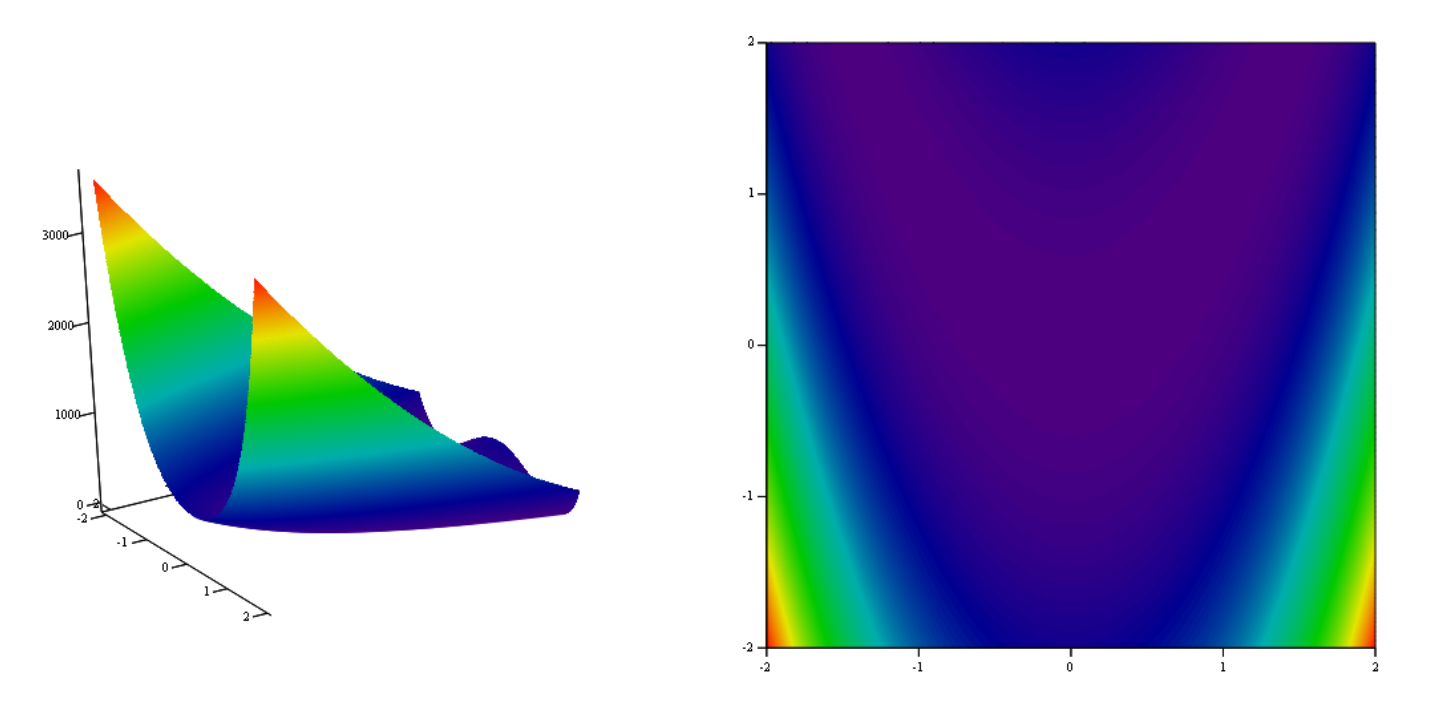
\includegraphics[width=16cm, height=8cm]{Rozenbrock}

    \subsubsection{Формула}
    \begin{gather*}
        f(x)=\sum_{i=1}^{n-1}\left(100\left(x_{i+1}-x_i^2\right)^2+\left(1-x_i\right)^2\right)
    \end{gather*}

    \subsubsection{Результаты тестирования}

    \begin{tabular}{ |p{2cm}|p{2cm}|p{3cm}|p{2cm}|p{4cm}|  }
        \hline
        n & точность & метод         & время   & значение            \\
        \hline
        2 & $10^-3$  & Golden ratio  & 1.12 ms & 0.16956582889643249 \\\cline{2-5}
        & $10^-3$  & Moore-Skelboe & 155 ms  & 0.16036252999621464 \\
        \hline
        3 & $10^-3$  & Golden ratio  & 5.95 ms & 0.259397310396006   \\\cline{2-5}
        & $10^-3$  & Moore-Skelboe & 3.99 s  & 0.11254106932659813 \\
        \hline
        4 & $10^-3$  & Golden ratio  & 17 ms   & 0.28064340055794645 \\\cline{2-5}
        & $10^-3$  & Moore-Skelboe & 8.75 s  & 0.11734786681147619 \\
        \hline
        5 & $10^-3$  & Golden ratio  & 27.3 ms & 0.2830939134564683  \\\cline{2-5}
        & $10^-3$  & Moore-Skelboe & 15.6 s  & 0.11851270446807871 \\
        \hline
        6 & $10^-3$  & Golden ratio  & 40.4 ms & 0.29047947563212634 \\\cline{2-5}
        & $10^-3$  & Moore-Skelboe & 24.5 s  & 0.11879389607067276 \\
        \hline
        7 & $10^-3$  & Golden ratio  & 49.2 ms & 0.29064024190256904 \\\cline{2-5}
        & $10^-3$  & Moore-Skelboe & 35.6 s  & 0.1136410373197746  \\
        \hline
        8 & $10^-3$  & Golden ratio  & 18.5 ms & 0.33244082803407593 \\\cline{2-5}
        & $10^-3$  & Moore-Skelboe & 41.7 s  & 0.14015453688727936 \\
        \hline

    \end{tabular}

    \subsection{Функция Экли}

    \subsubsection{График функции при $n=2$}
    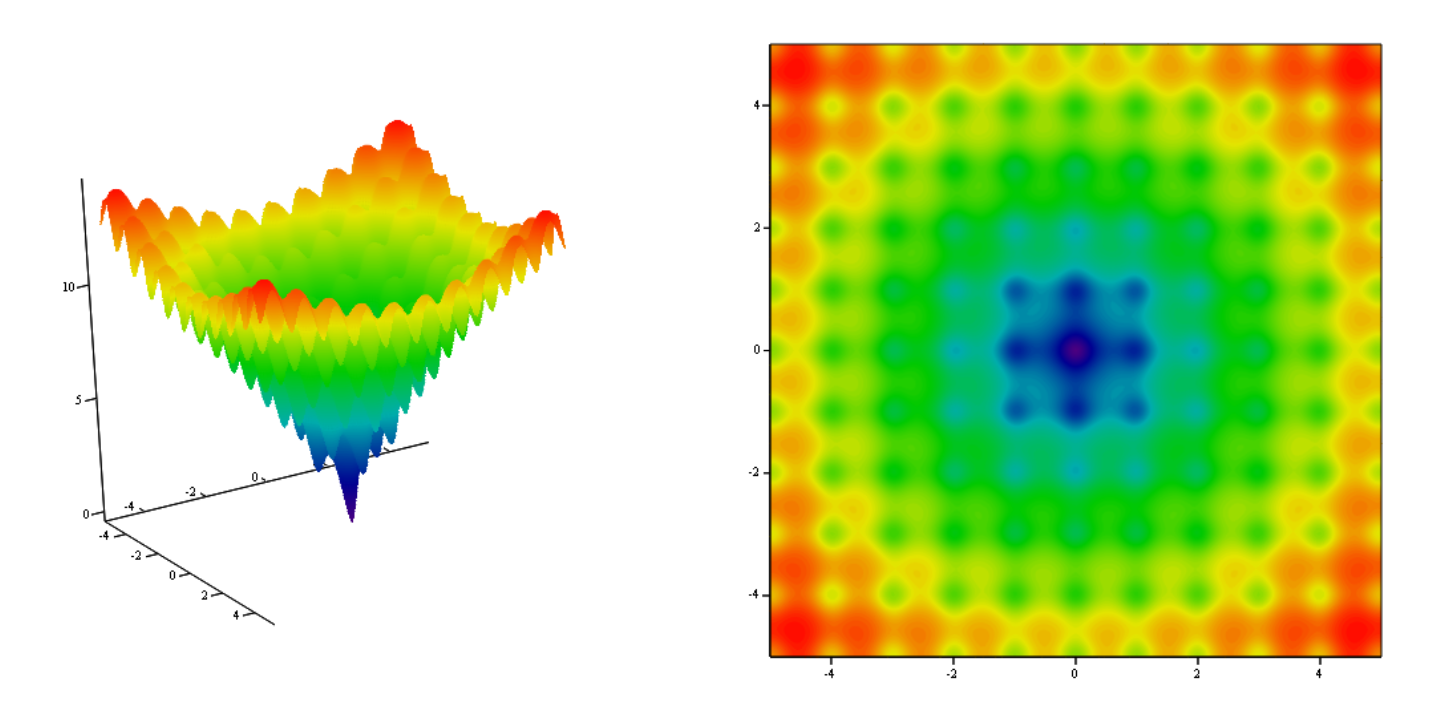
\includegraphics[width=16cm, height=8cm]{Ackley}

    \subsubsection{Формула}
    \begin{gather*}
        f(x)=20+e-20 e^{-0.2 \sqrt{\frac{1}{n} \sum_{i=1}^n x_i^2}}-e^{\frac{1}{n} \sum_{i=1}^n \cos \left(2 \pi \cdot x_i\right)}
    \end{gather*}

    \subsubsection{Результаты тестирования}

    \begin{tabular}{ |p{2cm}|p{2cm}|p{3cm}|p{2cm}|p{4cm}|  }
        \hline
        n  & точность & метод         & время   & значение               \\
        \hline
        5  & $10^-3$  & Golden ratio  & 2.41 ms & -4.440892098500626e-16 \\\cline{2-5}
        & $10^-3$  & Moore-Skelboe & 553 ms  & 0.0012256630393632229  \\
        \hline
        20 & $10^-3$  & Golden ratio  & 9.06 ms & 3.5744545080266543     \\\cline{2-5}
        & $10^-3$  & Moore-Skelboe & 1.35 s  & 0.0012256630393632229  \\
        \hline
        20 & $10^-3$  & Golden ratio  & 30.6 ms & 3.5744545080266543     \\\cline{2-5}
        & $10^-3$  & Moore-Skelboe & 3.41 s  & 0.0012256630393632229  \\
        \hline
        30 & $10^-3$  & Golden ratio  & 58.5 ms & 3.574454508026655      \\\cline{2-5}
        & $10^-3$  & Moore-Skelboe & 6.23 s  & 0.0012256630393645551  \\
        \hline
        40 & $10^-3$  & Golden ratio  & 84.1 ms & 3.574454508026654      \\\cline{2-5}
        & $10^-3$  & Moore-Skelboe & 10.6 s  & 0.0012256630393632229  \\
        \hline
        50 & $10^-3$  & Golden ratio  & 124 ms  & 3.5744545080266525     \\\cline{2-5}
        & $10^-3$  & Moore-Skelboe & 14.9 s  & 0.0012256630393618906  \\
        \hline

    \end{tabular}

    \subsection{Функция Гриванка}

    \subsubsection{График функции при $n=2$}
    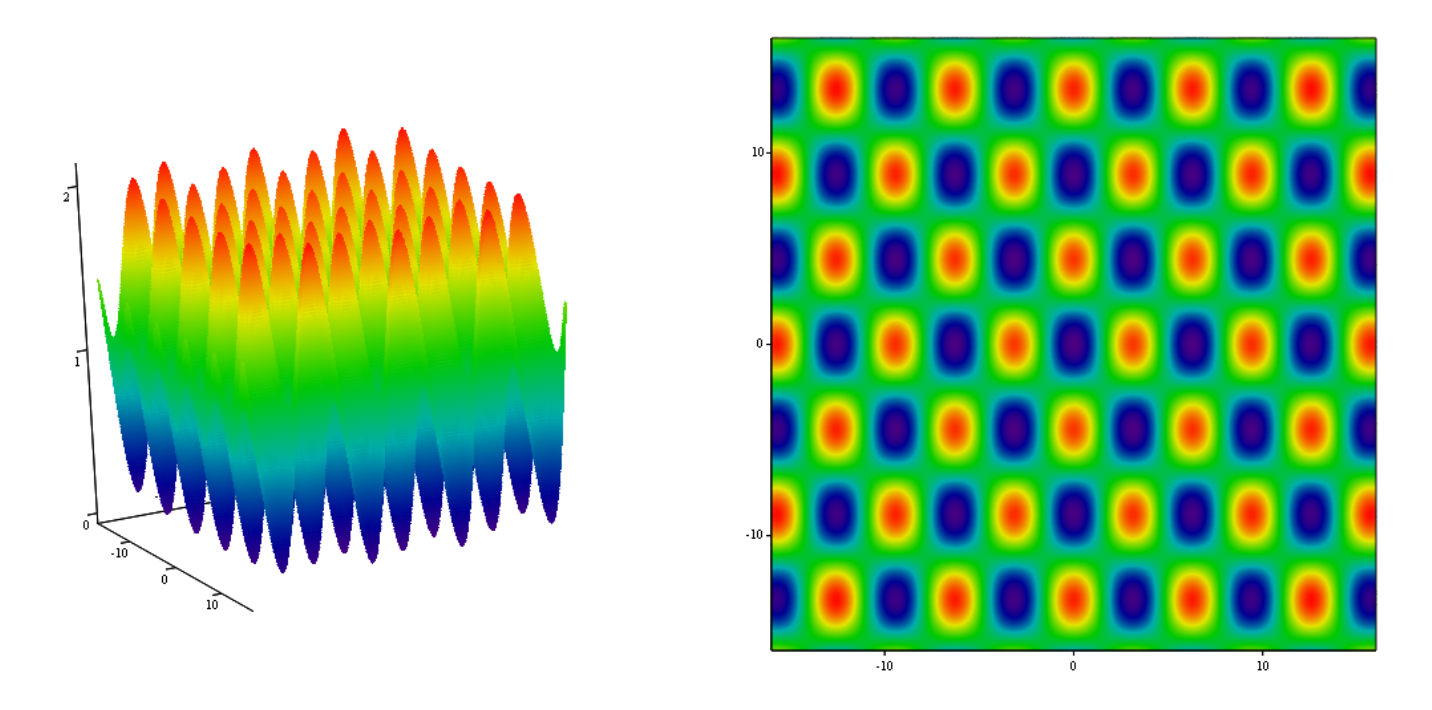
\includegraphics[width=16cm, height=8cm]{Grivank}

    \subsubsection{Формула}
    \begin{gather*}
        f(x)=\sum_{i=1}^n \frac{x_i^2}{4000}-\prod_{i=1}^n \cos \left(\frac{x_i}{\sqrt{i}}\right)+1
    \end{gather*}

    \subsubsection{Результаты тестирования}

    \begin{tabular}{ |p{2cm}|p{2cm}|p{3cm}|p{2cm}|p{4cm}|  }
        \hline
        n  & точность & метод         & время   & значение               \\
        \hline
        5  & $10^-3$  & Golden ratio  & 2.41 ms & 0.009864698515380743   \\\cline{2-5}
        & $10^-3$  & Moore-Skelboe & 183 ms  & 1.0644240466817223e-07 \\
        \hline
        10 & $10^-3$  & Golden ratio  & 6.05 ms & 0.009864698515380743   \\\cline{2-5}
        & $10^-3$  & Moore-Skelboe & 739 ms  & 1.3662353537391425e-07 \\
        \hline
        20 & $10^-3$  & Golden ratio  & 21.4 ms & 0.009864698515380743   \\\cline{2-5}
        & $10^-3$  & Moore-Skelboe & 2.44 s  & 1.6799845647952338e-07 \\
        \hline
        30 & $10^-3$  & Golden ratio  & 40.2 ms & 0.009864698515380743   \\\cline{2-5}
        & $10^-3$  & Moore-Skelboe & 5.16 s  & 1.867295605917363e-07  \\
        \hline
        40 & $10^-3$  & Golden ratio  & 59.3 ms & 0.009864698515380743   \\\cline{2-5}
        & $10^-3$  & Moore-Skelboe & 9.09 s  & 2.0016648982768004e-07 \\
        \hline
        50 & $10^-3$  & Golden ratio  & 84.4 ms & 0.009864698515380743   \\\cline{2-5}
        & $10^-3$  & Moore-Skelboe & 14 s    & 2.1067470723501458e-07 \\
        \hline

    \end{tabular}

    \subsection{Функция Швефеля}

    \subsubsection{График функции при $n=2$}
    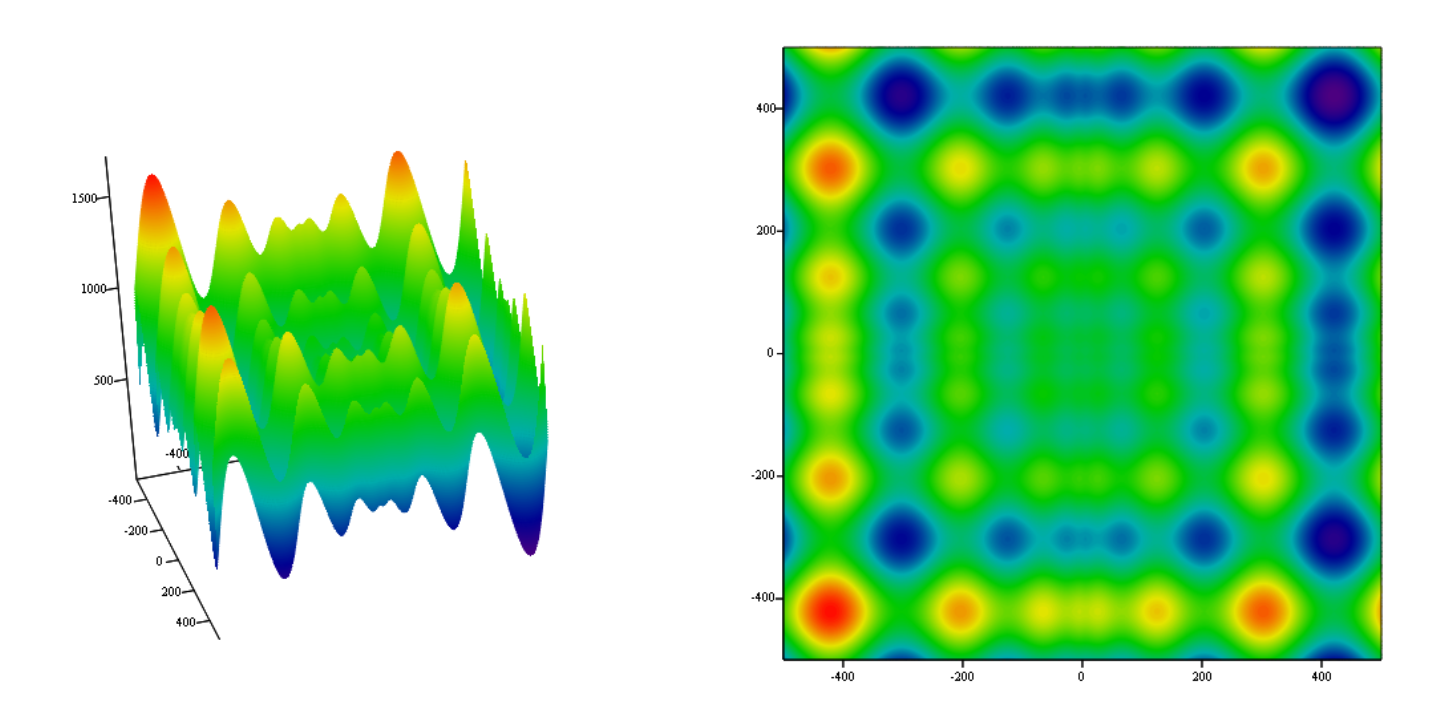
\includegraphics[width=16cm, height=8cm]{Shvefel}

    \subsubsection{Формула}
    \begin{gather*}
        f(x)=418.9829 n-\sum_{i=1}^n\left(x_i \sin \left(\sqrt{\left|x_i\right|}\right)\right)
    \end{gather*}

    \subsubsection{Результаты тестирования}

    \begin{tabular}{ |p{2cm}|p{2cm}|p{3cm}|p{2cm}|p{4cm}|  }
        \hline
        n & точность & метод         & время   & значение               \\
        \hline
        2 & $10^-3$  & Golden ratio  & 721 µs  & 236.8766946858181      \\\cline{2-5}
        & $10^-3$  & Moore-Skelboe & 4.98 s  & 2.5455285594944144e-05 \\
        \hline
        3 & $10^-3$  & Golden ratio  & 800 µs  & 355.3150420287272      \\\cline{2-5}
        & $10^-3$  & Moore-Skelboe & 9.41 s  & 3.8182928392416216e-05 \\
        \hline
        4 & $10^-3$  & Golden ratio  & 1.44 ms & 473.7533893716363      \\\cline{2-5}
        & $10^-3$  & Moore-Skelboe & 15 s    & 5.091057118988829e-05  \\
        \hline
        5 & $10^-3$  & Golden ratio  & 1.4 ms  & 592.1917367145454      \\\cline{2-5}
        & $10^-3$  & Moore-Skelboe & 22 s    & 6.363821398736036e-05  \\
        \hline
        6 & $10^-3$  & Golden ratio  & 2.19 ms & 710.6300840574543      \\\cline{2-5}
        & $10^-3$  & Moore-Skelboe & 31.1 s  & 7.636585655745876e-05  \\
        \hline
        7 & $10^-3$  & Golden ratio  & 1.88 ms & 829.0684314003631      \\\cline{2-5}
        & $10^-3$  & Moore-Skelboe & 40 s    & 8.909349912755715e-05  \\
        \hline
        8 & $10^-3$  & Golden ratio  & 4.92 ms & 947.5067787432718      \\\cline{2-5}
        & $10^-3$  & Moore-Skelboe & 52 s    & 0.00010182114169765555 \\
        \hline

    \end{tabular}












    \newpage


    \section{Список литературы}
    \begin{itemize}
        \item Сергиенко А. Б. Тестовые функции для глобальной оптимизации.
        \item Пантелеев, Летова: Методы оптимизации в примерах и задачах.
        \item Ratschek, Rokne. New Computer Methods for Global Optimization.
    \end{itemize}


    \section{Первые выводы}
    Проведя тестирование на 6 функциях, на 5 из них (кроме Розенброка) наш алгоритм справлялся и находил глобальный минимум, когда классические методы находили совсем не то что нужно, что логично. Но так как других методов, с которыми можно сравнить результат моей работы не нашлось, то сравнивал с таким.


\end{document}